\documentclass[11pt]{article}
\usepackage[letterpaper, margin=2cm]{geometry}
\usepackage{titlesec}
\usepackage{mdframed}
\usepackage[dvipsnames]{xcolor} % for color names, must be loaded before tikz
\usepackage{ifthen}
\usepackage{comment}
\usepackage{fancyhdr}
\usepackage{fancyvrb}
\usepackage{titling}
\usepackage{hyperref}
\usepackage{enumitem}
\usepackage{tikz}
\usepackage{amsmath, amssymb, amsthm}

\providecommand{\due}{}
\lhead{Virtualization} \rhead{The University of Texas}
\lfoot{\due} \cfoot{} \rfoot{Page \thepage}
\renewcommand{\footrulewidth}{0.4pt}
\pagestyle{fancy}

% Eliminates the spacing in the title that remains from the empty author section.
\preauthor{}
\postauthor{}

\titleformat{\section}[runin]{\large\bfseries}{\thesection .}{3pt}{}
\titleformat{\subsection}[runin]{\bfseries}{\thesubsection)}{3pt}{}
\renewcommand\thesubsection{\alph{subsection}}

% Defines the solution environment. Toggle solutions between true and false to either show or hide solutions. Also, the solution environment takes an optional argument of arbitrary text to be inserted in the solution header.
\newboolean{solutions}
\setboolean{solutions}{true}
\ifthenelse{\boolean{solutions}}
{\newenvironment{solution}{\begin{mdframed}[skipbelow=0pt, linecolor=White, backgroundcolor=Green!10]\textbf{Solution:}}{\end{mdframed}}}
{\excludecomment{solution}}

\allowdisplaybreaks

\begin{document}

\title{Virtualization\\Pre-lab Questions --- \#0}
\date{\due}

\maketitle

\noindent \textbf{Point total:} 12
\\ All homework assignments are weighted equally in the final grade. 
Point values are unique to each lab assignment.

\textbf{Note:} For all problems which ask you to explain your reasoning or show your work, 
you do not need to show every step of each calculation, 
but the answer should include an explanation \emph{written with words} of what you did.  
Even when work is not required to be shown, it’s a good idea to include anyways so that 
you can earn partial credit.

\section{Question [2 points]}

Which register contains the return value of the function? 
What is the value you see? Is this an address or a constant value?

\begin{solution}
\%rax contains the return value of the function. The value we see is:
 `rax            0x8004209610     549825058320'.
 It generally can be both an address or a value, currently it is a value 
 but since the function is void eventually it will be the value 0x0. 
\end{solution}


\section{Question [2 points]}

Which register contains the next assembly instruction to execute? 
What is the value you see? Is this an address or a constant value?

\begin{solution}
The register \%rip contains the next instruction to execute. 
The value we see is: `rip            0x8004209610     0x8004209610 env\_pop\_tf'. 
It is the address of the next instruction, not a constant value. 
\end{solution}


\section{Question [2 points]}

Using the answer from the previous question, what are the next 5 instructions that will be executed? 
What are the hex codes of those functions? (hint: see $display$ in gdb)
As you may notice, the function calls a c function 
\begin{verbatim} __asm __volatile() \end{verbatim}
The asm statement allows you to include assembly instructions directly within C code. 
The volatile keyword simply tells the assembler not to optimize this instruction away.

\begin{solution}
The next 5 instructions (found by running `x/5i \$pc`) are:

\begin{BVerbatim}
1. 0x8004209610 <env_pop_tf>:   push   \%rbp
2. 0x8004209611 <env_pop_tf+1>: mov    \%rsp,\%rbp
3. 0x8004209614 <env_pop_tf+4>: push   \%rbx
4. 0x8004209615 <env_pop_tf+5>: sub    \$0x18,\%rsp
5. 0x8004209619 <env_pop_tf+9>: mov    \%rdi,-0x18(\%rbp)
\end{BVerbatim}

The hex codes are:

\begin{BVerbatim}
1. 0x55
2. 0x48
3. 0x89
4. 0xe5
5. 0x53
\end{BVerbatim}
\end{solution}


\section{Question [2 points]}

Explain what the following assembly instructions are doing, line by line.

\begin{center}
\begin{BVerbatim}
push   \%rbp
mov    \%rsp,\%rbp
push   \%rbx
sub    \$0x18,\%rsp
\end{BVerbatim}
\end{center}

\begin{solution}
    \begin{enumerate}
        \item push \%rbp: This command is pushing the value of the \%rbp register onto the stack. 
        Essentially saving the old base pointer value so when the function returns it can be restored.

        \item mov \%rsp, \%rbp: Copy the value of the \%rsp register to the \%rbp register. \%rsp points to the top 
        of the stack so this effectivelly creates a new stack frame. 

        \item push \%rbx: Push the value of the \%rbx register to the stack. 

        \item sub \$0x18, \%rsp: Subtract the value 0x18 from the \%rsp register. This tells the stack pointer to 
        allocate space.
    \end{enumerate}

In summary, we saved the old base \%rbp, established a new stack frame, saved the old \%rbx, and allocated space 
for variables. Basically set up the stack for a function. \%rbp and \%rbx are callee-saved so we had to manually 
save them. 
\end{solution}


\section{Question [2 points]}

Using the $stepi$ functionality in GDB, which will execute one instruction at a time, 
what do the registers look like after the above instructions are executed?

\begin{solution}
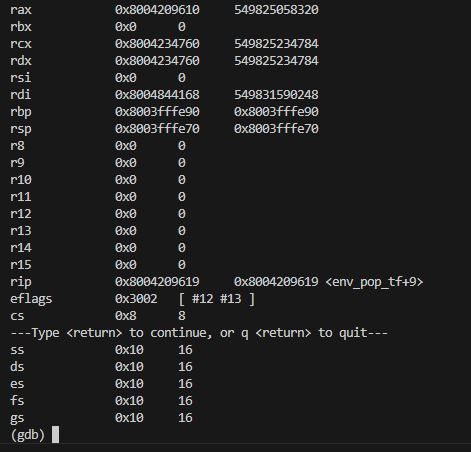
\includegraphics{register_output.jpg}
\end{solution}


\section{Question [2 points]}

Notice that the first line of assembly in the \texttt{\_\_asm\_\_volatile\(\)} 
call is \texttt{movq \%0,\%\%rsp}. If you were to change this line to \texttt{movq \$0,\%\%rsp} 
(notice the \$), you would see an error in GDB the next time \texttt{rsp} is used. 
Why would this change introduce an error?

\begin{solution}
rsp is used to keep track of the current position in the stack. `movq \%0, \%\%rsp' is valid 
because we are setting the stack pointer to the value contained in the address `\%0'. 
However, `\$0' is an actual value, not an address. Therefore if we set \%rsp to 0, 
we'll be pointing to address 0 which is not a valid address since it is usually protected. 
\end{solution}


\end{document}

